% Historical report: superseded by docs/memory.md and
% docs/MEMORY_LIFECYCLE_TUTORIAL.md for the current memory-v2 write path.
\documentclass[11pt]{article}

\usepackage[margin=1in]{geometry}
\usepackage{amsmath,amssymb}
\usepackage{booktabs}
\usepackage{longtable}
\usepackage{xcolor}
\usepackage{enumitem}
\usepackage{tikz}
\usetikzlibrary{arrows.meta,positioning,calc,fit,backgrounds,shapes.geometric}
\usepackage{graphicx}
\usepackage{float}
\usepackage{listings}
\usepackage[hidelinks]{hyperref}
\usepackage[htt]{hyphenat}
\emergencystretch=2em

\definecolor{cardblue}{HTML}{2166AC}
\definecolor{evgreen}{HTML}{1B7837}
\definecolor{harmred}{HTML}{B2182B}
\definecolor{coldgray}{HTML}{7F7F7F}
\definecolor{codebg}{HTML}{F4F4F2}

\newcommand{\code}[1]{\texttt{\small #1}}
\newcommand{\card}{c}
\newcommand{\gain}{g}

\lstdefinestyle{py}{
  basicstyle=\ttfamily\scriptsize,
  backgroundcolor=\color{codebg},
  keywordstyle=\color{cardblue}\bfseries,
  commentstyle=\color{coldgray}\itshape,
  stringstyle=\color{evgreen},
  language=Python,
  showstringspaces=false,
  breaklines=true,
  frame=leftline,
  framerule=1.2pt,
  rulecolor=\color{cardblue},
  xleftmargin=1.2em,
  aboveskip=6pt, belowskip=4pt,
  morekeywords={Protocol,class,def,async,await,self,None,str,int,float,bool,list,dict,tuple}
}

\title{\textbf{GigaEvo Memory: How a Run Becomes a Card}\\[2pt]
\large Extraction, the librarian, the admission gate, gain-event attribution, and the OOP seams}
\author{GigaEvo --- \code{gigaevo/memory/write}}
\date{Rebuilt memory subsystem (PR \#294, branch \code{refactor/memory-rebuild})}

\begin{document}
\maketitle

\begin{abstract}
The write side of GigaEvo memory turns a \emph{completed} (or in-progress)
evolutionary run into durable, reusable \emph{cards} and the \emph{gain-event}
evidence the read side later scores. This document traces the full chain: which
programs are eligible to become memory (extraction), how a parent$\to$child diff
is reconciled by an LLM into 0..$N$ clean idea cards (the librarian), how a
single harm gate admits or refuses each card and journals every verdict (the
admission ledger), how top-fitness programs become exemplar cards, how each
card is credited with \emph{use-attributed, base-relative} gain events
(the substrate the reputation posterior consumes), and how periodic
consolidation folds near-duplicates. It closes with a reference section on the
object-oriented seams --- the Protocols and \code{\_target\_} injection points ---
where the system is designed to be extended. Every mechanism below is grounded
verbatim in \code{gigaevo/memory/write/\{writer,extraction,librarian,admission,
stats,merge,eviction,consolidation\}.py} and \code{cards.py}. It is the companion
to \emph{``How a Card Earns Its Place in the Prompt''} (the read-side report);
the two meet at the gain event.
\end{abstract}

\section*{Terminology}
\addcontentsline{toc}{section}{Terminology}

The write side has its own vocabulary; every term is defined here at first use
and reused unchanged.

\begingroup
\setlength{\parskip}{0pt}
\begin{description}[leftmargin=1.4em, itemsep=1.5pt, parsep=0pt, style=unboxed]
  \item[\textcolor{cardblue}{Card}] the one banked memory unit
    (\code{cards.Card}). \emph{Kind} \code{insight} is a distilled text lesson;
    kind \code{program} is an exemplar (a strong past solution + its code). One
    frozen Pydantic model; behavior forks on \code{card.kind}, never on type.
  \item[\textcolor{cardblue}{Record}] a \code{ProgramRecord} --- the slice of a
    program the write path needs (id, fitness, parents, normalized mutation
    changes, base parent + its code), with no stage results or raw execution
    data. Extraction turns eligible programs into records.
  \item[\textcolor{cardblue}{Base parent}] the specific parent the mutator
    anchored a child to (1-based \code{base\_parent}). The diff, the gain
    baseline, and use-attribution are all measured \emph{against the base}, not
    against whichever parent the selector happened to list first.
  \item[\textcolor{evgreen}{Librarian}] the LLM-first idea-write path: it fetches
    the nearest existing cards, runs the reconcile agent over the diff, and routes
    each authored card to the gate. The only write-time dedup arbiter on the idea
    path.
  \item[\textcolor{evgreen}{Reconcile (NEW / DUPLICATE / MERGE)}] the per-card
    verdict the reconcile agent returns for each authored idea: \emph{admit fresh}
    (NEW), \emph{bump an existing card's provenance} (DUPLICATE), or \emph{union
    onto an existing card} (MERGE).
  \item[\textcolor{harmred}{Admission gate}] \code{CardAdmissionGate} --- the sole
    harm authority. Four methods (\code{admit}, \code{merge},
    \code{bump\_provenance}, \code{sweep}) decide admit-or-reject and record every
    verdict to the ledger. It owns \emph{harm}, nothing else.
  \item[\textcolor{harmred}{Write ledger}] \code{write\_ledger.jsonl} --- the
    append-only audit trail (\code{write\_ledger.v1}) answering ``what happened to
    the card I submitted, and why'' for every gate verdict.
  \item[\textcolor{cardblue}{Gain event}] one \code{ContextualGain}: a card's
    signed, base-relative fitness effect on \emph{one} credited child, tagged with
    the base parent's metrics as decision context. A card's whole track record is
    its list of gain events --- and it is exactly what the read side scores. (This
    is the one object the two reports share; the read report colors it identically.)
  \item[\textcolor{evgreen}{Use-attribution}] the credit rule: a card is credited
    for a child only when it was both \emph{selected} for the child's base parent
    \emph{and} \emph{declared applied} by the mutator --- the intersection.
  \item[\textcolor{evgreen}{Restamp}] each sweep recomputes every card's gain
    events from the full program pool and overwrites them. Events are
    authoritative, not incremental.
  \item[\textcolor{harmred}{Harm eviction}] deleting a card whose injection
    posterior is \emph{confidently harmful}. The verdict is the read side's
    reputation, inverted into the write path through the \code{CardScorer}
    Protocol.
  \item[\textcolor{cardblue}{Consolidation}] a throttled background pass that
    folds near-duplicate idea cards the greedy online path let through, one
    \code{every\_n} cards written.
  \item[\textcolor{cardblue}{Sweep / increment}] one call of the write pipeline
    over a set of programs. The post-run hook runs one at the end; the live hook
    runs them mid-run on a cadence.
  \item[\textcolor{cardblue}{Store}] the shared \code{MemoryStore} (bank $+$ vector
    index). The reader reads the same instance the writer fills, so a write is
    visible to the next read with no cross-view reconciliation.
\end{description}
\endgroup

\section{The write pipeline at a glance}
\label{sec:glance}

One sweep (\code{MemoryWriter.\_run\_increment\_locked}) is a five-stage pipeline
over a completed run's program pool. Figure~\ref{fig:flow} shows the whole
system: an \emph{authoring tier} (top) turns diffs and exemplars into cards
through the LLM and the gate, and a \emph{bookkeeping tier} (bottom) turns the
program pool into the gain-event evidence and prunes harm --- pure functions of
the pool, no LLM.

\begin{figure}[ht]
\centering
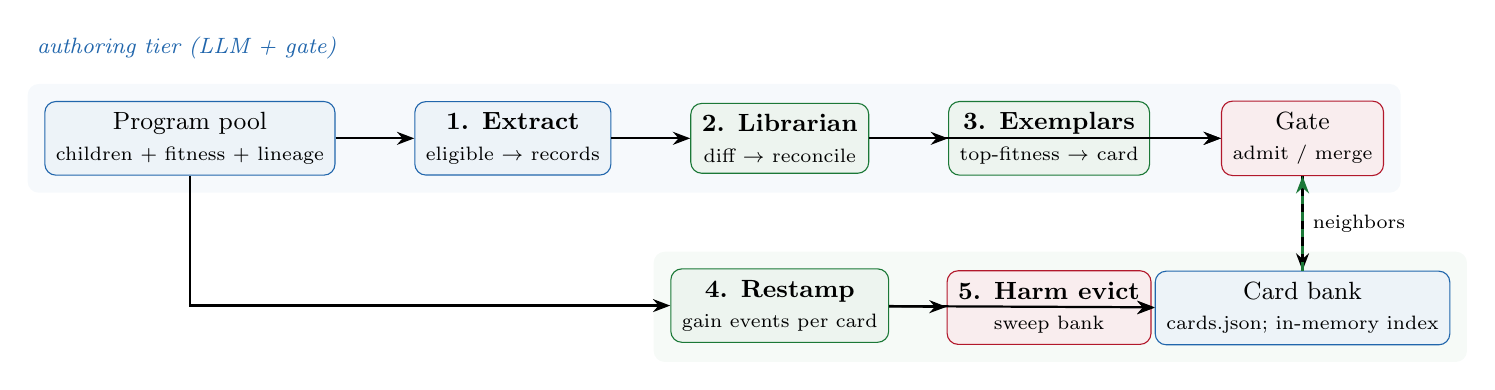
\begin{tikzpicture}[
  font=\small,
  box/.style={draw, rounded corners, align=center, inner sep=4pt, minimum height=8mm},
  src/.style={box, fill=cardblue!8, draw=cardblue},
  ev/.style={box, fill=evgreen!8, draw=evgreen},
  hz/.style={box, fill=harmred!8, draw=harmred},
  arr/.style={-{Stealth[length=2.2mm]}, thick},
  darr/.style={-{Stealth[length=2.2mm]}, thick, dashed, draw=evgreen}]
% authoring tier
\node[src] (pool) {Program pool\\{\scriptsize children $+$ fitness $+$ lineage}};
\node[src, right=10mm of pool] (extract) {\textbf{1. Extract}\\{\scriptsize eligible $\to$ records}};
\node[ev, right=10mm of extract] (lib) {\textbf{2. Librarian}\\{\scriptsize diff $\to$ reconcile}};
\node[ev, right=10mm of lib] (exemplar) {\textbf{3. Exemplars}\\{\scriptsize top-fitness $\to$ card}};
\node[hz, right=9mm of exemplar] (gate) {Gate\\{\scriptsize admit / merge}};
% bookkeeping tier
\node[ev, below=12mm of lib] (stats) {\textbf{4. Restamp}\\{\scriptsize gain events per card}};
\node[hz, below=12mm of exemplar] (evict) {\textbf{5. Harm evict}\\{\scriptsize sweep bank}};
\node[src, below=12mm of gate] (bank) {Card bank\\{\scriptsize cards.json; in-memory index}};

\draw[arr] (pool) -- (extract);
\draw[arr] (extract) -- (lib);
\draw[arr] (lib) -- (exemplar);
\draw[arr] (lib) -- (gate);
\draw[arr] (exemplar) -- (gate);
\draw[arr] (gate) -- (bank);
\draw[arr] (pool.south) |- (stats.west);
\draw[arr] (stats) -- (evict);
\draw[arr] (stats) -- (bank);
\draw[arr] (evict) -- (bank);
\draw[darr] (bank.north) -- (gate.south) node[midway,right,font=\scriptsize]{neighbors};
\begin{scope}[on background layer]
  \node[fill=cardblue!4, rounded corners, fit=(pool)(extract)(lib)(exemplar)(gate), inner sep=6pt] (top) {};
  \node[fill=evgreen!4, rounded corners, fit=(stats)(evict)(bank), inner sep=6pt] {};
\end{scope}
\node[anchor=west, font=\footnotesize\itshape, cardblue] at ([yshift=4.5mm]top.north west) {authoring tier (LLM + gate)};
\end{tikzpicture}
\caption{The write pipeline. Stages 1--3 are the authoring tier --- extraction is a
pure metadata pass that only returns records, while the librarian and exemplar
stages call the LLM and route \emph{their} cards through the harm gate; stages 4--5
attribute gain events and prune harm as pure functions of the program pool. The bank
is the shared store the reader reads; it is also the \emph{neighbor source} (dashed)
that feeds dedup at every authoring step.}
\label{fig:flow}
\end{figure}

Only stages 2--3 spend LLM tokens (extraction is a pure metadata pass). \emph{Model}
failures degrade rather than propagate, but by three different routes, not one: a
stalled ingest is dropped for retry on a later sweep, a failed reconcile call admits
the raw note \emph{verbatim} (not a drop), and failed neighbor retrieval falls back
to no-dedup. What still aborts the sweep is cancellation or an uncaught store/gate
error --- the honest invariant is ``specific model failures degrade; cancellation and
store/gate faults abort'' (\S\ref{sec:faults} gives the exact table). Stages 4--5 are
deterministic given the pool.

\paragraph{The funnel.} Not every program becomes a card. Figure~\ref{fig:funnel}
shows the eligibility narrowing: from the full pool down to the parented,
strictly-valid, not-yet-seen children that extraction turns into records, and
separately the top-fitness slice that becomes exemplar cards.

\begin{figure}[ht]
\centering
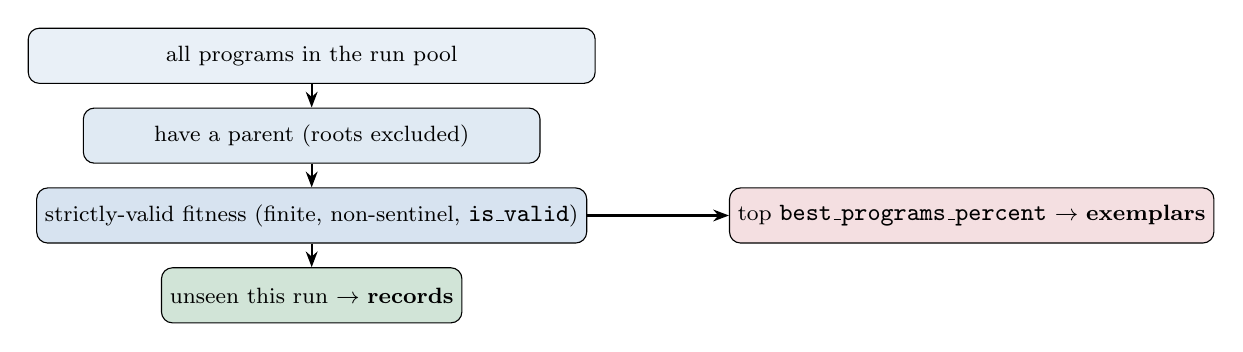
\begin{tikzpicture}[font=\footnotesize,
  lvl/.style={draw, rounded corners, align=center, minimum height=7mm, inner sep=3pt},
  arr/.style={-{Stealth[length=2mm]}, thick}]
\node[lvl, fill=cardblue!10, minimum width=72mm] (a) {all programs in the run pool};
\node[lvl, fill=cardblue!14, minimum width=58mm, below=3mm of a] (b) {have a parent (roots excluded)};
\node[lvl, fill=cardblue!18, minimum width=44mm, below=3mm of b] (c) {strictly-valid fitness (finite, non-sentinel, \code{is\_valid})};
\node[lvl, fill=evgreen!20, minimum width=30mm, below=3mm of c] (d) {unseen this run $\to$ \textbf{records}};
\node[lvl, fill=harmred!14, minimum width=30mm, right=18mm of c] (e) {top \code{best\_programs\_percent} $\to$ \textbf{exemplars}};
\draw[arr] (a)--(b); \draw[arr] (b)--(c); \draw[arr] (c)--(d);
\draw[arr] (c.east)-- ++(6mm,0) |- (e.west);
\end{tikzpicture}
\caption{Two eligibility funnels over one pool. Idea cards come from every
eligible mutation diff; exemplar cards come from the top-fitness slice. The two
are independent --- an exemplar program is usually also an idea-diff record.}
\label{fig:funnel}
\end{figure}

\section{Extraction: which programs become memory}
\label{sec:extract}

\code{ProgramRecordExtractor.extract} (\code{write/extraction.py}) is pure with
respect to the store and the LLM --- it only reads program metadata. It applies
three eligibility filters and normalizes the mutator's free-form output into a
typed record.

\subsection{Eligibility}

A program is skipped unless all three hold:
\begin{enumerate}[leftmargin=1.6em, itemsep=1pt]
  \item \textbf{Parented.} \code{prog.lineage.parents} is non-empty. Root
    (seed) programs have no diff to reconcile.
  \item \textbf{Strictly-valid fitness.}
    \code{metrics\_context.strict\_fitness(prog.metrics, fitness\_key)} is not
    \code{None} --- the metric is present, its \code{is\_valid} flag is
    positive, and the value is finite and not the failure sentinel. A missing
    key returns \code{None} and \emph{filters the program out} rather than minting
    a default; and \code{fitness\_key} defaults to the task's primary metric, so a
    stray hard-coded \code{"fitness"} key on a task whose primary metric differs
    can never silently zero every gain.
  \item \textbf{Unseen.} \code{prog.id} is not already in \code{\_seen\_ids}. The
    live hook and the post-run hook share one extractor, so this is what stops a
    program being re-ingested across overlapping sweeps.
\end{enumerate}

\subsection{The base parent and the diff}

Multi-parent mutation means ``the parent'' is ambiguous. The mutator records a
1-based \code{base\_parent} index in its \code{mutation\_output}; \code{program\_to\_record}
resolves it (\code{base\_index = base\_parent - 1}), falling back to the first
parent when out of range --- matching \code{freeze\_base\_parent\_snapshot} on
the mutation side. The base parent's \emph{code} is looked up from the pool and
attached, because the reconcile agent diffs \emph{child against base}, and in
$\ge 2$-parent rewrite mode the base may not be parent 0.

\paragraph{Validating the mutator's changes.} The mutator already emits
\code{changes} as a strict \code{list[MutationChange]} --- each item is exactly
\code{description} $+$ \code{explanation}, pinned by the mutation agent's
structured-output schema. Extraction re-validates that payload into a
\code{list[Improvement]} (the same two fields) straight off the stored
\code{model\_dump}; there is no free-form parsing and no keyword-scanning. Bad
data raises rather than being silently coerced --- the typed boundary is the
producer's schema, not a downstream heuristic.

\subsection{Seen-id bookkeeping and rollback}

\code{extract} marks every returned record's id \code{seen} \emph{before} the
librarian runs. If an ingest later times out or is cancelled, the orchestrator
calls \code{extractor.forget(\{id\})} to un-see it, so a later sweep retries the
record instead of losing its idea forever (\S\ref{sec:faults}). The
\code{parent\_code} lookup deliberately draws from \code{posterior\_programs}
(the full pool) when the live hook capped the working \code{programs} window ---
mutation parents are usually older archive elites outside the newest window, and
without the full pool the librarian would lose the parent code its diff needs and
silently degrade to ungrounded authoring.

\section{The librarian: an LLM authors clean cards from a diff}
\label{sec:librarian}

For each record, \code{Librarian.ingest\_idea} (\code{write/librarian.py}) runs
three steps: \textbf{retrieve} nearest cards, \textbf{reconcile} the diff into
authored cards, \textbf{route} each to the gate by decision.

\begin{figure}[ht]
\centering
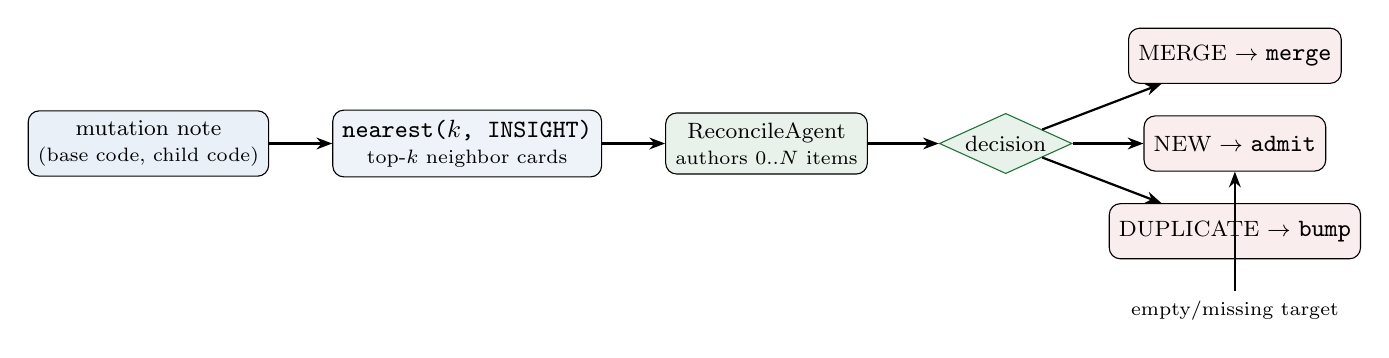
\begin{tikzpicture}[font=\footnotesize, node distance=6mm,
  b/.style={draw, rounded corners, align=center, inner sep=3.5pt, minimum height=7mm},
  dec/.style={draw, diamond, aspect=2.2, align=center, inner sep=1pt, fill=evgreen!10, draw=evgreen},
  arr/.style={-{Stealth[length=2mm]}, thick}]
\node[b, fill=cardblue!10] (note) {mutation note\\{\scriptsize (base code, child code)}};
\node[b, fill=cardblue!8, right=8mm of note] (near) {\code{nearest($k$, INSIGHT)}\\{\scriptsize top-$k$ neighbor cards}};
\node[b, fill=evgreen!10, right=8mm of near] (agent) {ReconcileAgent\\{\scriptsize authors 0..$N$ items}};
\node[dec, right=9mm of agent] (d) {decision};
\node[b, fill=harmred!8, right=9mm of d] (new) {NEW $\to$ \code{admit}};
\node[b, fill=harmred!8, below=4mm of new] (dup) {DUPLICATE $\to$ \code{bump}};
\node[b, fill=harmred!8, above=4mm of new] (mrg) {MERGE $\to$ \code{merge}};
\draw[arr] (note)--(near); \draw[arr] (near)--(agent); \draw[arr] (agent)--(d);
\draw[arr] (d)--(new); \draw[arr] (d)--(dup); \draw[arr] (d)--(mrg);
\draw[arr] (dup.south) -- ++(0,-4mm) -| node[near start,below,font=\scriptsize]{empty/missing target} (new.south);
\end{tikzpicture}
\caption{One \code{ingest\_idea}. The agent is the only dedup arbiter; a
DUPLICATE/MERGE whose target is empty or already gone falls back to NEW rather
than dropping the idea.}
\label{fig:ingest}
\end{figure}

\paragraph{Retrieval is insight-only.} The neighbors fetched are
\code{CardKind.INSIGHT} only: an idea is never a near-duplicate of a program
exemplar, and the agent must not be offered program ids as merge targets.

\paragraph{No cosine gate on the idea path.} There is deliberately \emph{no}
embedding-distance threshold anywhere on the idea write path. Raw mutation notes
and authored prose sit too far apart in embedding space for a cosine gate to
fire on real twins, and same-lever cards average only $\sim 0.78$ cosine
similarity on this geometry --- any threshold strong enough to catch duplicates
would also force-merge distinct levers. Recall is pure top-$k$ by rank; the LLM
is the precision arbiter. (The one exception is the exemplar path,
\S\ref{sec:exemplars}, which has no LLM arbiter and so keeps a small
\code{program\_twin\_eps} distance cut.)

\paragraph{An LLM failure never drops the idea.} If neighbor retrieval fails,
the agent simply runs with no context. If the reconcile call itself fails, the
librarian admits the raw note \emph{verbatim} as a fresh card --- a degraded
card, never a silent drop. Authored output is capped at
\code{max\_cards\_per\_diff} (default 3) so one noisy diff cannot flood the bank.

\section{The admission gate and the write ledger}
\label{sec:gate}

\code{CardAdmissionGate} (\code{write/admission.py}) is the whole admission
surface --- four methods, one concern (harm), one side effect (the ledger). It
does \emph{not} dedup (the librarian does) and does not author prose.

\begin{longtable}{@{}p{0.20\textwidth}p{0.74\textwidth}@{}}
\toprule
\textbf{Method} & \textbf{What it does} \\
\midrule
\endhead
\code{admit(card)} & Harm-check via the evictor; if harmful, delete any known-id
copy and journal \code{rejected\_harm}. Otherwise \code{store.save} and journal
\code{added} (new id) or \code{updated} (known id replaced). \\
\code{merge(target, card)} & Fetch the insight target; \code{merge\_cards} folds
\code{card} onto it (\S\ref{sec:merge}); harm-check the \emph{union}; on pass
\code{apply\_merges} and journal \code{merged}. The ledger's \code{incoming\_id}
is the \emph{submitted} card's, captured before the fold overwrites it. \\
\code{bump\_provenance(target, child)} & DUPLICATE ruling: append the child id to
an existing insight card's \code{programs} tuple, no LLM, no new card. Journal
\code{updated}. \\
\code{sweep()} & Snapshot the bank, ask the evictor which cards are confidently
harmful, delete each and journal \code{evicted}. \\
\bottomrule
\end{longtable}

\paragraph{The ledger is the contract.} \code{WriteLedgerRecord}
(\code{write\_ledger.v1}) is the one externally-consumed artifact of the write
path. Every row carries \code{incoming\_id}, \code{final\_id} (merge target for
merges, \code{""} if dropped), an \code{outcome} the gate actually emits ---
\{\code{added, updated, merged, rejected\_harm, evicted}\} --- and a human-readable
\code{reason}. Recording must never block the write path: any ledger failure is
logged and swallowed. Store save/merge events fire separately and automatically
through the store (\code{MEMORY\_STORE\_WRITE}, carrying the live
\code{bank\_count}), so the gate adds no counters of its own.

\section{Merge semantics: never lose evidence}
\label{sec:merge}

Folding one idea card into another must never drop the survivor's accumulated
evidence. \code{merge\_cards} (\code{write/merge.py}) is pure --- no I/O, no LLM
--- and both the gate and the consolidation pass route their unions through it.

\begin{longtable}{@{}p{0.26\textwidth}p{0.68\textwidth}@{}}
\toprule
\textbf{Field} & \textbf{Merge rule} \\
\midrule
\endhead
\code{id}, \code{category} & Kept from the \emph{target} (the survivor). \\
\code{description}, \code{explanation\_summary} & \code{replace\_description}
picks the winner: a MERGE takes the author's curated prose; a provenance bump
keeps the target's. \\
\code{keywords} & \emph{Replaced} by the author's curated union on a MERGE (so a
de-bloated set is not re-inflated). A provenance bump (DUPLICATE) does not route
through \code{merge\_cards} at all --- it only appends the child id to
\code{programs}, leaving prose and keywords untouched. \\
\code{programs}, \code{gain\_events} & Always unioned --- the accumulated
provenance and track record of \emph{both} cards survive. \\
\code{absorbed\_ids} & The folded-away incoming id (and any ids it had itself
absorbed) become aliases of the survivor, so a child that credited the now-gone
id re-aliases here at restamp (\S\ref{sec:restamp}). Blank ids and the
survivor's own id are never added. \\
\code{task\_description[\_summary]} & Fall back to whichever side carries them. \\
\bottomrule
\end{longtable}

The \code{absorbed\_ids} alias chain is what makes merges safe across restamps:
a child frozen at birth with a card id that is later merged away still credits
that id, which no longer exists in the bank --- the alias lets the survivor
re-collect that attribution instead of orphaning it.

\section{Program exemplars: capturing strong solutions}
\label{sec:exemplars}

In parallel with idea authoring, \code{\_author\_exemplars} banks a
\code card for each of the top
\code{best\_programs\_percent} programs (\code{MetricsContext.top\_valid\_programs}
resolves the slice, respecting the fitness direction). Exemplar authoring differs
from idea authoring in three ways:

\begin{itemize}[leftmargin=1.6em, itemsep=1pt]
  \item \textbf{Cached by program id.} \code{author\_program} first checks the
    bank for \code{program-<id>} with non-empty prose; a re-selected exemplar
    never re-pays the LLM.
  \item \textbf{Identity-keyed.} The card id is \code{program-<id>} --- stable, so
    re-admission flows to the gate as an \code{updated}, not a duplicate.
  \item \textbf{Twin dedup by distance + fitness.} Two \emph{different} programs
    that converge on the same strategy would bank two near-identical exemplars.
    \code{admit\_program} asks the neighbor source for a different-id program card
    within \code{program\_twin\_eps} cosine distance; if one exists it keeps only
    the strictly-higher-fitness exemplar (deleting the banked twin, or dropping
    the incoming one). This is the \emph{only} distance threshold in the entire
    write path, precisely because the exemplar path has no LLM arbiter.
\end{itemize}

\section{Gain events: the evidence the read side scores}
\label{sec:gain}

This is the write side's core product and the bridge to the read-side report.
After authoring, every card is re-credited with the \emph{use-attributed,
base-relative} gain events it earned across the pool
(\code{write/stats.py}). The read side computes \emph{all} per-card statistics
--- the Beta posterior, the harm count, the magnitude --- from exactly these
events; the write side's job is to produce them correctly.

\subsection{Use-attribution: who gets credit}

A card is credited for a child only at the \emph{intersection} of two frozen
facts (\code{compute\_contextual\_gains}):
\[
\text{credited}(\card) \;=\; \underbrace{\{\text{cards selected for the child's base parent}\}}_{\code{base\_selected\_ids}}
\;\cap\; \underbrace{\{\text{cards the mutator declared applied}\}}_{\code{card\_ids\_used}}.
\]
This excludes two false-credit classes: a \emph{donor} card (used, but selected
for the \emph{other} parent) and a \emph{hallucinated} id (declared used but
selected for neither) both earn nothing. Children with no frozen base baseline
(\code{base\_fitness is None}) or empty \code{base\_selected\_ids} contribute
nothing at all.

\subsection{The gain value and the invalid case}

For a credited valid child the event's gain is the base-relative,
orientation-corrected delta,
\[
\gain \;=\; \begin{cases} f_{\text{child}} - f_{\text{base}} & \text{maximize} \\ f_{\text{base}} - f_{\text{child}} & \text{minimize,}\end{cases}
\]
so positive always means improvement. An \emph{invalid} child (evaluated and
judged invalid) instead emits one \emph{forced-harm} event --- gain $0.0$, flag
\code{invalid=True} --- per credited card: the magnitude is meaningless but the
trial counts against the card. The event's \code{DecisionContext} carries the
base parent's id, its full metric dict, and the child's creation time.
Figure~\ref{fig:gain} shows one card's events over the children of a single base
parent.

\begin{figure}[H]
\centering
\includegraphics[width=0.82\textwidth]{memwrite_gain.pdf}
\caption{One credited card's gain events over the children of one base parent.
Each valid child is one signed, base-relative event; the read side's strict sign
test (\code{k\_harm}) counts the strictly-negative ones; each invalid child adds
one forced-harm event pinned at $0$ and tagged \code{invalid}. The card stores
only these raw events --- reputation derives the posterior from them at read
time.}
\label{fig:gain}
\end{figure}

\subsection{Restamp: events are authoritative, not incremental}
\label{sec:restamp}

Each sweep, \code{CardStatsUpdater.update} recomputes the events for \emph{every}
card from the full pool and overwrites them (\code{stamp\_gain\_events}); only
cards whose event tuple actually changed are rewritten. A credited card carries
this sweep's events; an \emph{un}credited card has any stale events cleared. The
sweep also folds in events the pool still attributes to the card's
\code{absorbed\_ids} (\S\ref{sec:merge}).

\paragraph{The multiplicity subtlety.} Every invalid child of one base parent
emits a value-identical forced-harm event, and those are distinct \emph{trials}
that must all survive. But the absorbed-id fold must drop the \emph{one} event a
child contributes when it credited both the survivor and an absorbed id. The
resolution is object identity: \code{card\_gain\_events\_from\_programs} binds
\emph{one} \code{ContextualGain} object per child and appends it to every
credited id's list, so deduping the absorbed fold by \code{id(event)} keeps
distinct value-equal trials and drops only the genuinely shared one. Concretely:
card $A$ absorbed $B$; child $X$ credited \emph{both} $A$ and $B$ --- one shared
event object --- while child $Y$ credited only $A$ with its own separate object.
The fold keeps $Y$'s independent trial and drops $X$'s duplicate, even though both
gains may be numerically equal, because \code{id(event)} distinguishes the two
objects where value-equality cannot. This relies on receiving one sweep's
freshly-built pool --- the sole caller's contract.

\section{Harm eviction: pruning confidently-harmful cards}
\label{sec:evict}

The write path must not import the read system, yet the harm verdict \emph{is}
the read side's injection posterior. \code{eviction.py} inverts that dependency
with a Protocol:

\begin{lstlisting}[style=py]
class CardScorer(Protocol):
    def card_stats(self, card, context=None) -> CardStatsBlock | None: ...
    def is_confidently_harmful(self, block) -> bool: ...
\end{lstlisting}

The write module \emph{declares} the surface it needs; \code{read/reputation.py}'s
reputation models satisfy it structurally; the integration config wires one
shared instance into both sides. \code{HarmEvictor} evicts a card iff its
posterior is confidently harmful; \code{NullEvictor} never evicts (the
bank-maintenance twin of \code{memory=none} on the read side). Eviction runs once
per sweep, after the restamp, so it always judges the freshest evidence.

\section{Consolidation: cleaning up greedy drift}
\label{sec:consolidation}

The online librarian is greedy and order-dependent: two same-lever cards can
both enter as NEW if neither pulls the other into the reconcile agent's top-$k$
context at birth. Consolidation (\code{write/consolidation.py}) is the standard
drift fix --- run the \emph{same} nearest-card primitive over the whole bank,
surface each card's top-$k$ neighbors as merge \emph{candidates}, and let the
consolidate agent be the precision arbiter, folding a pair only when it rules
they name the same lever. Figure~\ref{fig:consolidation} shows the effect.

\begin{figure}[H]
\centering
\includegraphics[width=0.82\textwidth]{memwrite_consolidation.pdf}
\caption{Greedy online admission lets near-duplicates accrete (dashed);
a consolidation pass every \code{every\_n} cards folds them back toward the true
distinct-lever count (solid). The pass is idempotent --- a second run over a
deduped bank folds nothing.}
\label{fig:consolidation}
\end{figure}

Three details make the pass safe:
\begin{itemize}[leftmargin=1.6em, itemsep=1pt]
  \item \textbf{Deferred deletes.} Absorbed partners are deleted only in a
    \code{finally}, per-id and independently, so the bank is stable while
    neighbors are ranked and one partner's persist failure cannot leave others
    live-yet-folded (a permanent gain double-count).
  \item \textbf{Over-fetch past consumed.} Because deletion is deferred, the
    query card's own slot and this-pass consumed cards still occupy the index;
    the pass fetches $k + 1 + |\text{consumed}|$ so $k$ genuine candidates always
    reach the arbiter.
  \item \textbf{Content-keyed decline memo.} Every pair the agent declines is
    remembered by \code{(id, description)}, carried across passes, so a frequent
    cadence never re-pays the arbiter for a pair it already ruled on --- yet the
    ruling invalidates the moment either card's prose changes.
\end{itemize}

\code{ConsolidationScheduler} throttles this to one background pass per
\code{every\_n} cards, dispatched non-blocking but serialized under the shared
write lock so it never interleaves with a live sweep. \code{drain} awaits the
final pass at run end (bounded by a timeout, with a cancel grace) so
\code{asyncio.run}'s teardown cannot silently drop the last consolidation.

\section{Sweeps, the run lock, and the live hook}
\label{sec:sweeps}

\code{MemoryWriter} is an \code{IncrementalPostRunHook}. \code{on\_run\_complete}
runs one final increment over the whole pool, then drains consolidation.
\code{LiveMemoryRefreshHook} (\code{live\_memory\_hook.py}) wraps the \emph{same}
writer as a \code{post\_step\_hook} so the bank is also rebuilt mid-run, on a
cadence counted in ingestor sweeps that landed at least one program.

Two invariants govern the split:
\begin{itemize}[leftmargin=1.6em, itemsep=1pt]
  \item \textbf{One write lock.} The live hook and the post-run hook share one
    \code{asyncio.Lock}; overlapping sweeps would interleave store writes and
    dedup bookkeeping. Consolidation takes the same lock.
  \item \textbf{Window vs.\ posterior split.} The live hook may cap the librarian's
    working \code{programs} to the newest $N$ (to stay inside the engine's time
    budget) but \emph{always} passes the full set as \code{posterior\_programs}.
    Gain attribution needs intact child$\to$parent lineage; a capped window would
    sever it and collapse the intro-event population. A failed live refresh does
    \emph{not} advance the cadence marker, so the next landing sweep retries
    immediately.
\end{itemize}

\section{Fault tolerance: model failures degrade, cancellation aborts}
\label{sec:faults}

The write path treats the memory LLM as unreliable by construction, so every
\emph{model} failure has a defined degradation and none of them, on their own, stops
the sweep before stages 4--5 (evidence $+$ harm) --- the load-bearing, pure
correctness steps. The invariant is narrower than ``nothing aborts,'' though: a
\emph{cancellation} (task teardown) or an uncaught \emph{store/gate} error propagates
and \emph{does} abort the increment before restamp. The distinction is exactly the
first two versus the last row-group of the table below --- model faults are caught
and reduced to a lesser card; control-flow and persistence faults are not.

\begin{longtable}{@{}p{0.30\textwidth}p{0.64\textwidth}@{}}
\toprule
\textbf{Failure} & \textbf{Degradation} \\
\midrule
\endhead
Neighbor retrieval fails & Agent runs with no context; authoring proceeds. \\
Reconcile call fails & Raw note admitted verbatim as one card (never a drop). \\
Ingest times out (\code{ingest\_call\_timeout\_s}) & Record dropped, its id
\code{forget}-ten for retry next sweep; siblings, exemplars, restamp, harm sweep
still run. \\
Ingest cancelled (\code{BaseException}) & Id rolled back via \code{forget}, then
re-raised (cancellation propagates). \\
Exemplar authoring/admission fails & That exemplar skipped; the rest, the
restamp, and the harm sweep still run. \\
Ledger write fails & Logged and swallowed --- journaling never blocks the write. \\
Consolidation pass fails & Failure counted and logged; folds \emph{already}
committed this pass persist, and only their partners are deleted (the \code{finally}
fires deferred deletes for committed folds only) --- the in-flight, uncommitted fold
leaves no trace. \\
Task-summary LLM fails & Falls back to the full task description (or \code{""}). \\
\bottomrule
\end{longtable}

\section{A worked increment}
\label{sec:worked}

One post-run sweep over a small pool, end to end:

\begin{enumerate}[leftmargin=1.6em, itemsep=2pt]
  \item \textbf{Extract.} 40 programs $\to$ 12 are parented, strictly-valid, and
    unseen $\to$ 12 records. Each carries its base parent's id and code and a
    one-line note from its normalized \code{changes}.
  \item \textbf{Ingest.} Record \code{p-317}'s note ``vectorize the inner loop''
    retrieves 5 insight neighbors; the reconcile agent returns one MERGE onto
    \code{idea-vectorize-88} and one NEW. The gate folds the first (unioning
    provenance $+$ events, journal \code{merged}) and admits the second (journal
    \code{added}). Two more records DUPLICATE existing cards $\to$ two provenance
    bumps.
  \item \textbf{Exemplars.} The top 5\% (2 programs) author \code{program-317}
    and \code{program-402}; \code{program-402} is within \code{program\_twin\_eps}
    of a banked exemplar but scores lower $\to$ dropped.
  \item \textbf{Restamp.} Over the full pool, use-attribution credits 9 cards;
    \code{idea-vectorize-88} collects 4 valid-gain events and 1 forced-harm event
    (one invalid child that used it), folding in one event still attributed to an
    id it absorbed in step 2. \code{MemoryGainRestamp} is emitted with the
    per-card counts.
  \item \textbf{Harm sweep.} One card's posterior is now confidently harmful
    (all 6 of its trials regressed the base) $\to$ evicted, journal \code{evicted}.
  \item \textbf{Consolidate.} \code{writes\_since} crossed
    \code{consolidation\_every\_n}; a background pass folds one straggler
    near-duplicate and is drained before the loop tears down.
\end{enumerate}

The bank now holds the union of everything the run learned, each card carrying
exactly the gain events the read side needs to score it next run.

\section{Extension points: the OOP seams (reference)}
\label{sec:extensions}

The write system is assembled from small typed objects behind Protocols and
Hydra \code{\_target\_} nodes, precisely so behavior can be swapped or added
\emph{without} editing the orchestrator. This section is a reference map of where
to extend, and how. The guiding rule (a project convention) is: \emph{prefer a
new implementation behind an existing seam over a new field or branch on an
existing class.}

\subsection{Seam 1 --- a new eviction policy (\code{Evictor} Protocol)}

The gate consults an \code{Evictor} through a two-method Protocol:
\code{should\_evict(card)} runs per card at admission, and \code{sweep(cards)} runs
over the whole population each write sweep. \code{HarmEvictor} and \code{NullEvictor}
ship. A staleness evictor, an ``evict below a confidence floor'' variant, or the
capacity bound below is a new class and a one-line config swap --- no gate change.
Note the split: a population-wide budget can only be enforced in \code{sweep} (which
sees every card); \code{should\_evict} sees one card in isolation, so it can only ever
apply a per-card test. The listing below is illustrative pseudocode, not shipped code.

\begin{lstlisting}[style=py]
class CapacityEvictor:  # trims toward a soft budget on each sweep, NOT at admit
    def __init__(self, scorer: CardScorer, max_cards: int) -> None:
        self._scorer, self._max = scorer, max_cards
    def should_evict(self, card: Card) -> bool:      # admit-time: harm test only
        return self._scorer.is_confidently_harmful(self._scorer.card_stats(card))
    def sweep(self, cards: Sequence[Card]) -> list[str]:   # batch: harm + overflow
        harmful = [c.id for c in cards if self.should_evict(c)]
        survivors = [c for c in cards if c.id not in harmful]
        weakest = sorted(survivors, key=lambda c: len(c.gain_events))  # least evidence first
        overflow = weakest[: max(0, len(survivors) - self._max)]
        return harmful + [c.id for c in overflow]
\end{lstlisting}

\begin{center}\code{evictor: \{\_target\_: ...CapacityEvictor, scorer: \$\{ref:memory.reputation\}, max\_cards: 500\}}\end{center}

\subsection{Seam 2 --- a new harm/quality verdict (\code{CardScorer} Protocol)}

The evictor scores through \code{CardScorer}, satisfied structurally by the read
side's reputation. A different notion of ``bad'' --- a frequentist test, a
drift detector, an ensemble of reputations --- is a new scorer wired into
\emph{both} sides by reference, preserving the ``harm verdict $=$ read-side
posterior'' invariant without a write$\to$read import.

\subsection{Seam 3 --- a new storage backend (\code{MemoryStore} ABC / \code{NeighborSource})}

Everything above storage speaks the \code{MemoryStore} contract and the narrow
\code{NeighborSource} Protocol (\code{nearest(text, k, kind)}). \code{LocalMemoryStore}
(Chroma $+$ JSON bank) ships; \code{RemoteMemoryStore} is a skeleton. A new
backend --- a hosted vector DB, a shared team bank, an in-memory fake for tests
--- implements the ABC and is swapped in config. The librarian, gate, and
consolidation pass are backend-agnostic because they only ever call
\code{nearest} / \code{save} / \code{merge\_retire} / \code{snapshot}.

One thing that is \emph{not} a transparent config tweak, despite living in the store:
the embedding model and \code{embed\_scopes}. Each \code{LocalMemoryStore} keeps
process-local in-memory Chroma collections derived from its locked card-bank view.
It rebuilds them from \code{cards.json} at startup and after cross-process bank
refreshes, so changed embedding settings take effect on the next startup rebuild.

\subsection{Seam 4 --- a new authoring or arbiter agent (LLM agent factories)}

The librarian's reconcile agent, program author, task-summary agent, and the
consolidate agent are all built by factories and injected. A domain-specialized
reconcile prompt, a stricter merge arbiter, or a multilingual author is a new
prompt directory plus a factory --- the librarian and consolidation code are
unchanged because they depend on the agent's typed response, not its prompt.
(Convention: externalize prompts under \code{prompts/<name>/} with a
\code{\{task\_description\}} placeholder; never inline terse prompts.)

\subsection{Seam 5 --- new dedup thresholds (\code{DedupPolicy} value object)}

Every dedup knob --- reconcile context width, exemplar twin $\varepsilon$,
consolidation candidate width --- lives in one frozen \code{DedupPolicy} node, so
tuning is config, not code. A new dedup \emph{regime} (e.g.\ a two-stage
coarse/fine consolidation) adds fields here and reads them in the pass, without
scattering scalars across the librarian and scheduler.

\subsection{Seam 6 --- richer decision context (\code{DecisionContext} model)}

\code{DecisionContext} (base id, base metrics, timestamp) is explicitly ``the
extension point for richer contexting later.'' Adding the search cell, the
mutation archetype, or a resource cost lets a future \emph{context-aware}
reputation (already prototyped as BD-proximity on the read side) restrict a
card's evidence to matching contexts --- the write side just needs to stamp the
richer context onto each \code{ContextualGain}.

\subsection{Seam 7 --- a new card kind (\code{CardKind} $+$ kind-gated validator)}

Insight vs.\ exemplar is a \code{StrEnum} with a kind-gated model validator, not
a class hierarchy. A third kind --- say a \code{counterexample} card (a lever
that reliably \emph{hurts}, kept to steer the mutator away) --- is a new enum
member, its field-gating rule in the one validator, and an authoring path; every
\code{card.kind}-switching site is then a compile-time-visible place to handle
it. Keeping one \code{Card} type (no \code{AnyCard}, no subclass-per-kind) is a
deliberate design choice that makes this cheap.

\subsection{What is intentionally \emph{not} a seam}

Two things are deliberately singular and should not be multiplied: the
\textbf{admission gate} (exactly one harm authority, so every write has one
audited verdict) and the \textbf{restamp contract} (events are a pure function of
the pool, recomputed whole each sweep --- no incremental-update path, because
that is where double-counting bugs live). Extend around these, not through them.

\section{Parameter reference}
\label{sec:params}

Every knob a user touches on the write path, with its config location and
default.

\begin{longtable}{@{}p{0.30\textwidth}p{0.40\textwidth}p{0.22\textwidth}@{}}
\toprule
\textbf{Parameter} & \textbf{Config} & \textbf{Default} \\
\midrule
\endhead
Fitness metric key & \code{writer.fitness\_key} & \emph{primary metric} \\
Exemplar share & \code{writer.best\_programs\_percent} & \code{5.0} \\
Per-call LLM timeout & \code{writer.ingest\_call\_timeout\_s} & \code{300.0} \\
Consolidation cadence & \code{writer.consolidation\_every\_n} & \code{32} (\code{0} = off) \\
Reconcile context width & \code{dedup\_policy.online\_top\_k} & \code{5} \\
Cards per diff (cap) & \code{dedup\_policy.max\_cards\_per\_diff} & \code{3} \\
Exemplar twin distance & \code{dedup\_policy.program\_twin\_eps} & \code{0.05} \\
Consolidation candidates & \code{dedup\_policy.consolidation\_k} & \code{5} \\
Harm evictor / null & \code{memory.evictor} group & \code{harm} (\code{full}/\code{writer}) \\
Live refresh cadence & \code{LiveMemoryRefreshHook.refresh\_every} & \code{10} \\
Live window cap & \code{LiveMemoryRefreshHook.max\_programs\_per\_sweep} & \emph{unbounded} \\
\bottomrule
\end{longtable}

\vspace{1em}
\noindent\emph{Companion:} the read-side report \emph{``How a Card Earns Its
Place in the Prompt''} picks up exactly where \S\ref{sec:gain} leaves off ---
turning these gain events into a reputation, an expected value, and a Thompson
auction for the prompt slot.

\end{document}
